% P24 — slajdy na obronę. Budowanie: `cd slides && latexmk main.tex`.
% Wykresy i tabela metryk są brane z `results/` (te same pliki co w raporcie).
\documentclass[aspectratio=169,11pt]{beamer}

\usepackage{iftex}
\ifPDFTeX
  \usepackage[T1]{fontenc}
  \usepackage{lmodern}
\else
  \usepackage{fontspec}
\fi
\usepackage{amsmath,amssymb}
\usepackage{booktabs}
\usepackage[locale=DE]{siunitx}

\usetheme{default}
\usecolortheme{seahorse}
\setbeamertemplate{navigation symbols}{}
\setbeamertemplate{footline}[frame number]
\setbeamertemplate{itemize items}[circle]

\graphicspath{{../results/figures/}}

\title{Detekcja spamu na danych zaszyfrowanych\\kryptosystemem Pailliera}
\subtitle{Projekt 9 --- Privacy-Preserving Spam Detection}
\author{Krzysztof Śliwiński, Piotr Waluszek}
\institute{Politechnika Krakowska, Wydział Informatyki i Telekomunikacji}
\date{}

\begin{document}

\begin{frame}
  \titlepage
\end{frame}

\begin{frame}{Problem i model zagrożeń}
  \begin{itemize}
    \item Filtr antyspamowy w chmurze widzi treść każdej wiadomości.
    \item Cel: serwer klasyfikuje wiadomość, \alert{nie widząc jej treści ani wyniku}.
  \end{itemize}
  \vspace{0.5em}
  \textbf{Przeciwnik: honest-but-curious serwer}
  \begin{itemize}
    \item wykonuje protokół poprawnie, ale zapisuje i analizuje wszystko, co widzi;
    \item zna klucz publiczny, model, słownik i ekstrakcję cech (Kerckhoffs) $\Rightarrow$ może szyfrować dowolne wiadomości (\alert{CPA});
    \item jedyny sekret: klucz prywatny klienta.
  \end{itemize}
  \vspace{0.5em}
  \textbf{Kryteria sukcesu:} accuracy $> 94\%$, te same predykcje co model jawny (100\%), odszyfrowany wynik $==$ obliczenie jawne.
\end{frame}

\begin{frame}{Paillier i Naive Bayes}
  \begin{columns}[T]
    \begin{column}{0.48\textwidth}
      \textbf{Paillier} ($g = n + 1$)
      \[ \mathrm{Enc}(m) = (1+n)^m\, r^n \bmod n^2 \]
      \begin{align*}
        \mathrm{Enc}(m_1)\cdot\mathrm{Enc}(m_2) &= \mathrm{Enc}(m_1 + m_2)\\
        \mathrm{Enc}(m)^k &= \mathrm{Enc}(k\,m)
      \end{align*}
      \begin{itemize}
        \item losowe $r$ $\Rightarrow$ IND-CPA (przy DCRA);
        \item tylko funkcje liniowe z jawnymi współczynnikami.
      \end{itemize}
    \end{column}
    \begin{column}{0.48\textwidth}
      \textbf{Multinomial NB $\to$ log-odds}
      \[ \Delta(\mathbf{x}) = b + \sum_{i=1}^{k} w_i x_i \]
      \begin{itemize}
        \item $b = \log P(\text{spam}) - \log P(\text{ham})$
        \item $w_i = \log\theta_{\text{spam},i} - \log\theta_{\text{ham},i}$
        \item spam $\Leftrightarrow \Delta > 0$
      \end{itemize}
      \vspace{0.3em}
      $\Delta$ to iloczyn skalarny z jawnymi wagami $\Rightarrow$ \alert{da się policzyć na szyfrogramach}.
    \end{column}
  \end{columns}
\end{frame}

\begin{frame}{Protokół}
  \begin{enumerate}
    \item \textbf{Klient:} TF-IDF $\mathbf{x} \in [0,1]^k$, kodowanie $\tilde{x}_i = \lfloor S x_i \rceil$, wysyła $\mathrm{Enc}(\tilde{x}_i)$ dla \alert{wszystkich} $i$ (także zer).
    \item \textbf{Serwer:} $c_\Delta = \mathrm{Enc}(\tilde{b}) \cdot \prod_i \mathrm{Enc}(\tilde{x}_i)^{\tilde{w}_i} \bmod n^2$ \quad ($\tilde{w}_i = \lfloor S w_i \rceil$, $\tilde{b} = \lfloor S^2 b \rceil$).
    \item \textbf{Klient:} $\tilde{\Delta} = \mathrm{Dec}(c_\Delta)$; spam $\Leftrightarrow \tilde{\Delta} > 0$.
  \end{enumerate}
  \vspace{0.5em}
  \textbf{Kodowanie stałoprzecinkowe ($S = 10^6$), a nie float z \texttt{phe}:}
  \begin{itemize}
    \item każda wartość to \texttt{int} $\Rightarrow$ jawny wykładnik zawsze $0$ $\Rightarrow$ nic nie zdradza;
    \item obliczenie na liczbach całkowitych jest \alert{dokładne} --- wynik można porównać przez $==$;
    \item jeden szyfrogram wyniku na wiadomość: mniej pracy serwera, klient mniej wie o modelu.
  \end{itemize}
\end{frame}

\begin{frame}{Dane i metodyka}
  \begin{itemize}
    \item SMS Spam Collection (UCI): 5574 wiadomości $\to$ \alert{5171 po deduplikacji} (653 spam, 12,6\%).
    \begin{itemize}
      \item bez deduplikacji 12\% wiadomości testowych ma kopię w zbiorze treningowym.
    \end{itemize}
    \item Podział 80/20 stratyfikowany: 4136 train / 1035 test (131 spam), stały seed.
    \item Pipeline: TF-IDF $\to$ selekcja $\chi^2$ ($k$ cech) $\to$ Multinomial NB.
    \item Strojenie: 168 konfiguracji, 5-fold CV \alert{tylko na train}, wybór po F1 spamu \\
      $\Rightarrow$ unigramy, sublinear TF, $k = 1000$, $\alpha = 0{,}01$.
    \item Grupy kontrolne: jawny NB (float64), klasa większościowa, regresja logistyczna.
    \item Klucz 2048 bit, Apple M5 Pro, \texttt{phe} + \texttt{gmpy2}.
  \end{itemize}
\end{frame}

\begin{frame}{Wyniki klasyfikacji}
  \begin{columns}[c]
    \begin{column}{0.55\textwidth}
      \centering
      \resizebox{\textwidth}{!}{% Wygenerowane przez `python -m src.evaluate` — nie edytować ręcznie.
\begin{tabular}{@{}lccccc@{}}
\toprule
Model & Acc. & Prec. & Rec. & F1 & ROC-AUC \\
\midrule
Encrypted NB (Paillier) & 0.981 & 0.944 & 0.901 & 0.922 & 0.991 \\
Plaintext NB & 0.981 & 0.944 & 0.901 & 0.922 & 0.991 \\
Logistic regression & 0.980 & 0.923 & 0.916 & 0.920 & 0.986 \\
Majority class & 0.873 & 0.000 & 0.000 & 0.000 & 0.500 \\
\bottomrule
\end{tabular}
}
      \vspace{1em}
      \begin{itemize}
        \item wersja zaszyfrowana $=$ jawny NB we \alert{wszystkich} metrykach;
        \item 98,07\% $> 94\%$, +10,7 p.p. nad klasą większościową.
      \end{itemize}
    \end{column}
    \begin{column}{0.42\textwidth}
      \centering
      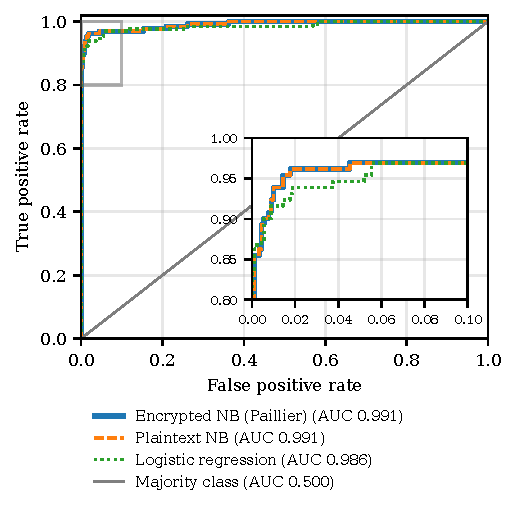
\includegraphics[width=\textwidth]{roc}
    \end{column}
  \end{columns}
\end{frame}

\begin{frame}{Zgodność i błąd kwantyzacji}
  \begin{itemize}
    \item Te same predykcje co jawny NB: \alert{1035 / 1035}.
    \item Odszyfrowany $\tilde{\Delta}$ $==$ to samo obliczenie jawnie na \texttt{int}: \alert{1035 / 1035}.
    \item Dwa pełne przebiegi (nowe klucze, nowe $r$): wyniki identyczne co do bitu.
  \end{itemize}
  \vspace{0.5em}
  \textbf{Kwantyzacja względem NB na floatach:}
  \begin{itemize}
    \item $|\tilde{\Delta}/S^2 - \Delta|$: maks. $1{,}35 \cdot 10^{-5}$, średnio $1{,}5 \cdot 10^{-6}$ (oszacowanie: $< 5 \cdot 10^{-5}$);
    \item najbliższa granicy wiadomość: $|\Delta| = 0{,}031$ --- ponad 2000$\times$ dalej;
    \item \alert{0 zmian znaku}.
  \end{itemize}
\end{frame}

\begin{frame}{Koszt i wybór $k$}
  \begin{columns}[c]
    \begin{column}{0.5\textwidth}
      \begin{itemize}
        \item Dominuje szyfrowanie: $k$ szyfrowań po ok. 4~ms (2048 bit) $\Rightarrow$ ok. 4~s na wiadomość na 1 rdzeń.
        \item Serwer ponad 50$\times$ taniej, odszyfrowanie ok. 1~ms.
        \item Wszystko liniowo w $k$; 3072 bit $\approx 3\times$ wolniej.
        \item 512~kB szyfrogramów na wiadomość ($k = 1000$).
        \item Cały zbiór testowy: ok. 10~min na 15 rdzeniach.
        \item F1 rośnie do $k \approx 750$--$1000$ (0,66 przy $k = 100$).
      \end{itemize}
    \end{column}
    \begin{column}{0.47\textwidth}
      \centering
      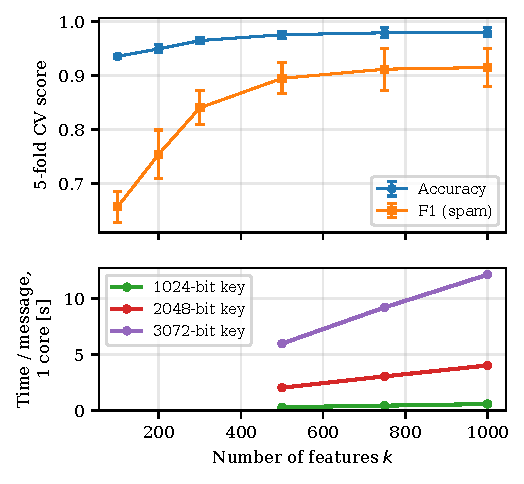
\includegraphics[width=\textwidth]{accuracy-vs-k}
    \end{column}
  \end{columns}
\end{frame}

\begin{frame}{Atak 1: klasyfikator na szyfrogramach}
  \begin{itemize}
    \item Serwer szyfruje 400 oznaczonych wiadomości (CPA) i uczy Random Forest na cechach szyfrogramów: najmłodszy bajt, $c \bmod 3, 5, 7$, długość, symbol Jacobiego $\left(\frac{c}{n}\right)$.
    \item $\left(\frac{c}{n}\right) = \left(\frac{r}{n}\right)$, bo $(1+n)^m \equiv 1 \pmod n$ --- zależy tylko od $r$.
  \end{itemize}
  \vspace{0.3em}
  \centering
  \begin{tabular}{@{}lcc@{}}
    \toprule
    Klasyfikator (5-fold CV) & Accuracy & F1 \\
    \midrule
    RF na szyfrogramach & 0,875 & 0,000 \\
    Klasa większościowa & 0,875 & 0,000 \\
    RF na jawnych cechach (kontrola) & 0,975 & 0,887 \\
    \bottomrule
  \end{tabular}
  \vspace{0.3em}
  \begin{itemize}
    \item Kontrola pokazuje, że 400 wiadomości wystarcza do nauki --- \alert{szyfrogramy nic nie zdradzają}.
  \end{itemize}
\end{frame}

\begin{frame}{Atak 2: dlaczego szyfrujemy także zera}
  \begin{itemize}
    \item Pokusa: wysyłać tylko niezerowe cechy z indeksami (mediana 3 z 1000 $\Rightarrow$ ok. 300$\times$ taniej).
    \item Wartości zaszyfrowane, ale serwer widzi, \alert{które słowa} są w wiadomości.
  \end{itemize}
  \vspace{0.3em}
  \centering
  \begin{tabular}{@{}lcc@{}}
    \toprule
    Co widzi serwer (zbiór testowy) & Accuracy & F1 \\
    \midrule
    Indeksy niezerowych pozycji (Bernoulli NB) & 0,984 & 0,931 \\
    Sama liczba niezerowych pozycji & 0,943 & 0,745 \\
    Jawny NB (odniesienie) & 0,981 & 0,922 \\
    Klasa większościowa & 0,873 & 0,000 \\
    \bottomrule
  \end{tabular}
  \vspace{0.3em}
  \begin{itemize}
    \item Same indeksy dają klasyfikator \alert{tak dobry jak nasz model} $\Rightarrow$ pełny wektor jest konieczny.
  \end{itemize}
\end{frame}

\begin{frame}{Ataki 3--4: losowe $r$ i jawny wykładnik}
  \textbf{Atak 3 --- niedeterminizm (6000 szyfrogramów, 451 różnych wartości):}
  \begin{itemize}
    \item losowe $r$ (\texttt{phe}): 6000 różnych szyfrogramów, odzyskane bez klucza: $\approx 0\%$;
    \item stałe $r$: 451 różnych szyfrogramów; najczęstszy to $\mathrm{Enc}(0)$, z niego serwer odzyskuje \alert{100\%} wartości.
  \end{itemize}
  \vspace{0.5em}
  \textbf{Atak 4 --- wykładnik \texttt{phe}:}
  \begin{itemize}
    \item przy kodowaniu float wykładnik zależy od rzędu wielkości wartości $\Rightarrow$ zdradza niezerowe pozycje (jak atak 2);
    \item kodowanie stałoprzecinkowe: wykładnik zawsze $0$ $\Rightarrow$ \alert{brak wycieku}.
  \end{itemize}
\end{frame}

\begin{frame}{Wnioski}
  \begin{itemize}
    \item NB to funkcja liniowa $\Rightarrow$ Paillier wystarcza; jeden szyfrogram wyniku na wiadomość.
    \item Wszystkie kryteria spełnione: accuracy 98,07\%, 100\% zgodności, dokładność $==$.
    \item Koszt po stronie klienta (ok. 4~s / wiadomość / rdzeń), ale równoległy i akceptowalny.
    \item Bezpieczeństwo zależy od szczegółów: \alert{losowe $r$}, \alert{pełny wektor}, \alert{kodowanie całkowite}.
    \item Ograniczenia: model jawny dla serwera, serwer pasywny, klient poznaje $\Delta$ (ryzyko ekstrakcji modelu).
  \end{itemize}
  \vspace{1em}
  \centering
  Kod i wyniki: \texttt{python -m src.run\_all}
\end{frame}

\end{document}
